\chapter{Eksperyment na danych właściwych (MRI FLAIR)}

\section{Opis danych}

Dane pochodzą z Uniwersytetu Duke'a (ang. Duke University). Są to zdjęcia głowy wykonane metodą obrazowania rezonansu magnetycznego w technice FLAIR (ang. fluid-attenuated inversion recovery) wraz z zaznaczonymi obszarami zmian nowotworowych. Obrazy mają rozmiar 256x256x3 pikseli, gdzie pierwszy kanał odpowiada momentowi przed wprowadzeniem kontrastu, trzeci po, a drugi jest właściwym zdjęciem. Maski mają rozmiar 256x256 pikseli o wartościach odpowiednio 255 dla komórek nowotworowych i 0 w przeciwnym wypadku. Na rysunku \ref{fig:medical_description} pokazane są zdjęcia z podziałem na kanały i odpowiadające im maski.

\begin{figure}[h!]
    \centering
    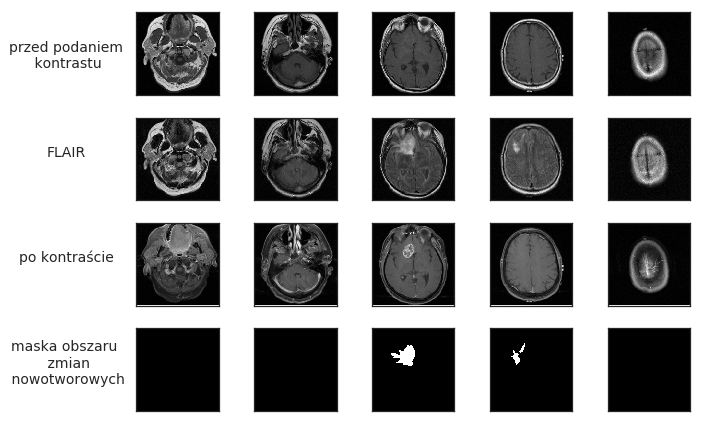
\includegraphics[width=0.8\textwidth]{images/medical_description}
    \caption{Przedstawienie konkretnych kanałów w próbce wraz z jego maską zmian}
    \label{fig:medical_description}
\end{figure}

Dane pogrupowane są dla 110 pacjentów ze zdiagnozowanym nowotworem. Na rysunku \ref{fig:medical_sample} zaprezentowałem zdjęcia pojedynczej osoby w trzech kanałach. Łącznie w zbiorze danych znajduje się 3929 par obrazów, przy czym jedynie $\sim1.02988\%$ pikseli zostało zidentyfikowanych jako komórki nowotworowe, co potwierdza obserwację odnośnie ich rzadkości.

\begin{figure}[h!]
    \centering
    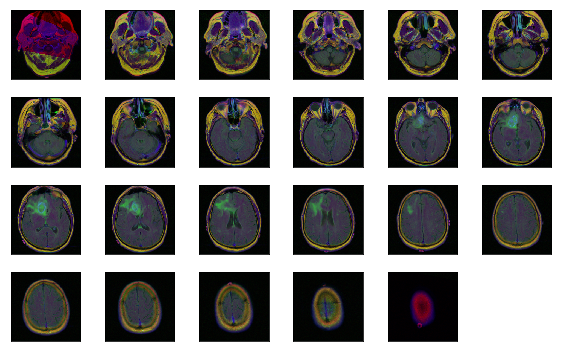
\includegraphics[width=0.8\textwidth]{images/medical_sample}
    \caption{Przykładowy zestaw obrazków dla pojedynczego pacjenta}
    \label{fig:medical_sample}
\end{figure}

\section{Wstępna obróbka}

Dane podzieliłem na 2 rozłączne zbiory ze względu na pacjentów w stosunku 70\% dla zestawu treningowego i 30\% dla testowego.

\subsection{Podział na mniejsze kawałki}

Danymi, które rzeczywiście mnie interesują są poszczególne komórki w mózgu. To co chciałbym umieć oceniać to ich patologiczność. Mam zamiar to robić na podstawie kontekstu w jakim się znajdują, czyli lokalnego sąsiedztwa na zdjęciu. W praktyce sprowadzi się to do utożsamiania wycinka obrazu rozmiaru $n$ x $n$ z wartością komórki leżącą w jego środku. W takim sensie chce podzielić zbiór danych na mniejsze kawałki, żeby każdej komórce odpowiadał jej kontekst. Jednak parametrem wymagającym ustalenia jest rozmiar takiego sąsiedztwa. Musze wiedzieć czy kawałek o danych wymiarach będzie zawierał wystarczającą ilość informacji potrzebnych do poprawnej klasyfikacji. Teoretycznie za kontekst mógłbym uznać cały obrazek, ale zależy mi też na ograniczeniu rozmiaru modelu i potrzebnej w związku z tym mocy obliczeniowej. Do wyznaczenia tej wartości skorzystam z podejścia nauki nadzorowanej, co może wydawać się sprzeczne z moją początkową deklaracją, ale ten krok służy jedynie we wsparciu wyboru optymalnego rozmiaru i nie jest wymagany.

Decyzję podejmę na podstawie rezultatów osiąganych przez modele takie jak regresja liniowa oraz splotowa sieć neuronowa dla następujących rozmiarów: 16, 22, 28, 32, 48, 64. Zakładam, że jeśli w jakimś przypadku dokładność będzie zadowalająca, to ilość obecnych informacji wystarczy do rekonstrukcji. Warto w tym miejscu wspomnieć, że przy takim podejściu muszę zrównoważyć dane w zbiorze treningowym, ponieważ aktualnie jednych jest około 100 razy mniej niż drugich. Rozwiążę to na takiej zasadzie, że w trakcie uczenia porcję danych wejściowych będę komponował losując połowę próbek z jednej klasy i połowę z drugiej. Może to wpłynąć negatywnie na obciążenie modelu, ale i tak ostateczna klasyfikacja będzie odbywać się z wykorzystaniem progu, co powinno zredukować ten błąd. Wyniki zaprezentowałem przy pomocy krzywych ROC na wykresie \ref{fig:supervised_patches}. Jak można zauważyć wszystkie rozważane rozmiary prezentują się równie dobrze, w związku z czym zdecydowałem się wybrać jako parametr liczbę 22.

\begin{figure}[h!]
  \centering
  \begin{subfigure}[b]{0.45\linewidth}
    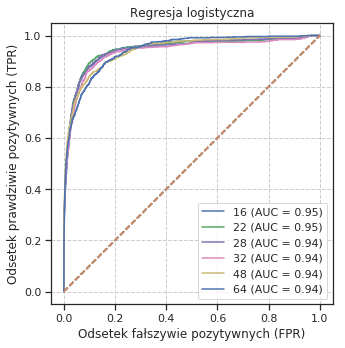
\includegraphics[width=\linewidth]{images/logreg_patch_roc_v2}
    %\caption{}
  \end{subfigure}
  \begin{subfigure}[b]{0.45\linewidth}
    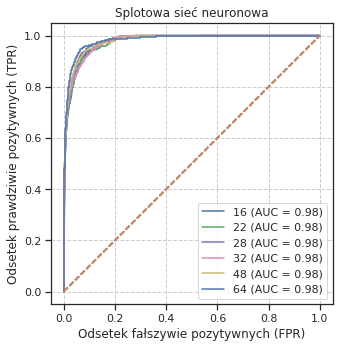
\includegraphics[width=\linewidth]{images/cnn_patch_roc_v2}
    %\caption{}
  \end{subfigure}
  \caption{Porównanie dokładności ze względu na różne rozmiary wycinków dla modeli uczonych metodą nadzorowaną}
  \label{fig:supervised_patches}
\end{figure}

Nie jest to oczywiście najlepsza metoda dla podejścia nadzorowanego, czym mogłoby być wykorzystanie architektury U-Net, ale powinno wystarczyć jako punkt odniesienia dla wymaganej ilości informacji w wycinku.

Dodatkowo w tym miejscu chciałbym wprowadzić słownictwo jakie będę używał do określania konkretnych próbek. Te odnoszące się da zmian nowotworowych będę nazywał pozytywnymi, a pozostałe negatywnymi.

\subsection{Dodatkowe analiza zbioru}

Po zdecydowaniu się na łatki rozmiaru 22 i przygotowaniu takiego zbioru postanowiłem dodatkowo przeanalizować jego zawartość w celu znalezienia trywialnych przypadków. Jednym z nich były kawałki znajdujące się poza czaszkę, które nigdy nie są nowotworowe. Będą to obrazki o niskiej łącznej sumie pikseli, co zaprezentowane jest na histogramie \ref{fig:pixel_sums}. Na początku można zauważyć sporą grupę przypadków niepatologicznych. Sprawdziłem, że minimalna wartość sumy dla klasy odpowiadającej nowotworom wynosi $56.5$. Przy tym założeniu usunąłem wszystkie obrazki u sumie mniejszej, niż $42.0$ co zmniejszyło ilość danych o $45.5\%$, pozbywając się trywialnych próbek. Dany próg będę oczywiście uwzględniał w późniejszej klasyfikacji.

\begin{figure}[h!]
    \centering
    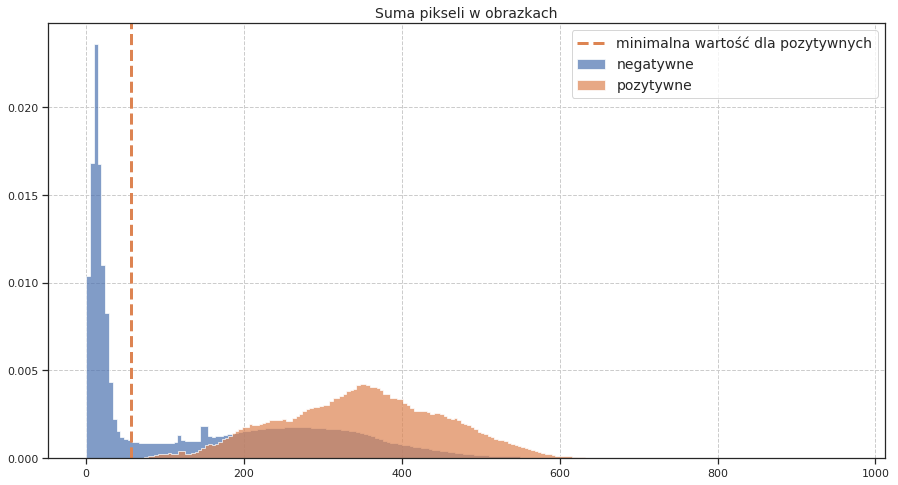
\includegraphics[width=1.0\textwidth]{images/pixel_sums_v3}
    \caption{Znormalizowany rozkład sum pikseli dla poszczególnych rodzajów próbek}
    \label{fig:pixel_sums}
\end{figure}
